\subsection{Iridescent}\label{2-fundamentacao-ferramentas-iridescent}

Iridescent~\cite{STAVROPOULOS-2013-Iridescent} é uma ferramenta \textit{standalone} que permite anotar descrições de serviços web de acordo com o padrão SAWSDL. As anotações são inseridas com base nas referências de termos de uma ontologia representada no formato OWL~\cite{W3C-2012-OWL}.

Por meio de uma interface gráfica de usuário, Iridescent permite que entidades identificadas na descrição de um serviço web sejam anotadas com os termos contidos na ontologia. A visualização de uma descrição de serviço web e uma ontologia ocorre por meio de uma representação visual no formato de árvore (\textit{tree-view}), semelhante ao \textit{plugin} Radiant~\cite{MILLER-VERMA-GOMADAM-SHETH-BREWER-2005-Radiant}.

Iridescent oferece recursos que automatizam parcialmente o processo de anotação semântica nos serviços web. A partir de um algoritmo de busca, conceitos de uma ontologia são sugeridos para os termos contidos em uma descrição de um serviço, servindo como um guia para o usuário. O usuário pode acatar ou não as sugestões da ferramenta. Iridescent também provê recursos para que os métodos \textit{Lifting Schema Mapping} e \textit{Lowering Schema Mapping} possam ser implementados e descritos no WSDL.

A utilização do recurso \textit{drag-and-drop} também auxilia o processo. O usuário pode arrastar elementos (conceitos) da representação visual de uma ontologia, do painel lateral direito, para um elemento WSDL presente no código disponibilizado pelo painel central. As anotações semânticas (SAWSDL) podem ser vistas diretamente no código WSDL/XML.

%O vínculo das anotações dos termos da ontologia com a descrição dos serviços web é realizado pela visualização do código WSDL/XML da descrição de serviço anotado semanticamente com a sintaxe SAWSDL~\cite{W3C-2007-SAWSDL}.

A \figurename~\ref{fig:iridescent} ilustra a interface gráfica de usuário de Radiant. Na lateral esquerda, encontram-se representados os elementos de uma ontologia. Na lateral direita, encontram-se representados os elementos WSDL. Finalmente, no centro, encontra-se a especificação WSDL anotada

\begin{figure}[h]
    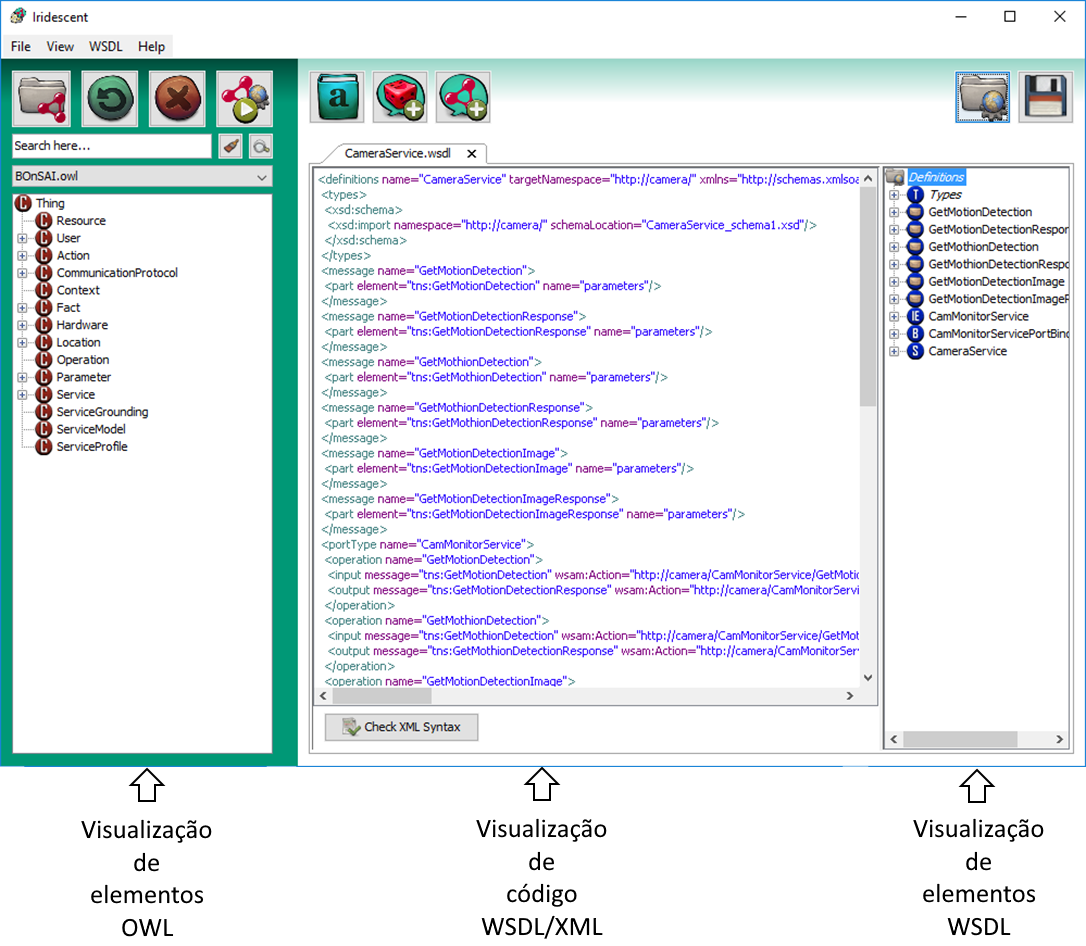
\includegraphics[scale=0.5]{2-fundamentacao-teorica/imagens/iridescent3.png}
    \centering
    \caption[Interface gráfica de usuário da ferramenta Iridescent.]{\textbf{Interface gráfica de usuário da ferramenta Iridescent.}}
    \label{fig:iridescent}
\end{figure}